\chapter{Introduction}
\section{Background}
Large Language Models (LLMs) represent a class of deep learning architectures trained on massive datasets, enabling them to comprehend and generate natural language with high versatility across domains \cite{shao2024survey}. As of 2025, approximately 67\% of organizations worldwide have adopted LLMs to support their operational workflows \cite{hostinger2025llm}. One of the most prominent applications of LLMs is in conversational agents or chatbots \cite{dam2024complete}. These systems often integrate retrieval pipelines \cite{gao2024retrieval} that extract domain-specific information from a database or knowledge store, and provide the retrieved content as context to the LLM for response generation. This architecture allows users to query against proprietary or organizational datasets using natural language and receive accurate, context-specific responses.

Meadow9+, a speech recognition application designed to record and transcribe long-duration meetings, is one such platform that integrates an LLM-powered chatbot to enable retrieval of information from meeting transcripts. The platform is widely utilised by corporations, welfare organizations, and medical professionals who rely on accurate transcription of meetings. Since meetings are where critical discussions and decisions take place, these transcripts effectively serve as a knowledge base for the organization. The integrated chatbot therefore plays a crucial role in extracting actionable insights from this knowledge, and the system must ensure both accuracy and responsiveness of the retrieval process.

Currently, the Meadow9+ chatbot processes full transcripts directly as input to the LLM. This design leads to two major limitations. First, excessively long inputs exacerbate the "lost in the middle" phenomenon \cite{liu2024lost}, where the LLM exhibits degraded performance when reasoning over information embedded in the middle sections of extended context windows. Second, longer context sequences increase computational overhead, thereby slowing inference and degrading user experience \cite{nvidia2023mastering}. Furthermore, transcription outputs often contain inaccuracies and inconsistencies \cite{metzger2024measuring}, and the current chatbot system lacks functionalities to handle noisy and ambiguous transcript data. These factors reduce usability and limit the effectiveness of the retrieval process for users who need quick and accurate access to meeting information.

\section{Motivations and Objectives}
Meeting transcripts only become truly valuable and actionable when users can quickly locate decisions, tasks, and explanations. However, Meadow9+ currently lacks an effective retrieval mechanism to support such use cases, which significantly limits the practical utility of long-duration transcripts. As mentioned, the existing Meadow9+ chatbot employs a monolithic prompting approach, in which entire transcripts are provided directly to the LLM. This design leads to high latency, increased computational overhead, and degraded user experience, rendering the system unreliable in real-world scenarios. Improving information retrieval within Meadow9+ therefore directly addresses a critical gap in the current system and has immediate applicability in real-world deployments.

This project presents an opportunity to apply modern information retrieval (IR) and LLM integration techniques beyond naive prompting. In particular, Retrieval-Augmented Generation (RAG) combines classical retrieval methods with generative models, enabling systems to retrieve relevant document segments before generation \cite{fan2024survey}. Furthermore, the project also enables exploration of advanced retrieval enhancements, including query preprocessing, phonetic encoding, and fuzzy matching.

Motivated by these considerations, this project aims to design and implement a comprehensive transcript retrieval system that improves both retrieval accuracy and end-to-end system performance for long meeting transcripts. Specifically, the objectives are:

\begin{itemize}
  \item Build a transcript retrieval pipeline that indexes long meeting transcripts into retrievable units and supports semantic retrieval via embeddings.
  \item Integrate retrieval into the chatbot using a RAG workflow to avoid full-transcript prompting, improving latency while maintaining answer quality.
  \item Develop a comprehensive evaluation pipeline to measure retrieval quality and end-to-end question answering performance using standard metrics, including hit-based metrics, reciprocal-rank metrics, and QA-style correctness metrics.
  \item Conduct empirical benchmarking comparing RAG against the existing pure LLM baseline under realistic conditions, with a focus on both accuracy and response latency.
  \item Explore extensible retrieval techniques tailored to noisy ASR transcripts, enabling efficient date-based and keyword-based retrieval in addition to chatbot-driven querying.
\end{itemize}

\section{Scope}
The scope of this project primarily focuses on the design and implementation of a RAG pipeline tailored for long-duration meeting transcripts. This includes developing appropriate transcript preprocessing strategies, such as chunking and embedding, to enable efficient and scalable retrieval from large textual documents. Particular emphasis is placed on handling the characteristics of long-form transcripts, where individual segments may vary in length and informational density, and ensuring that the resulting representations are suitable for downstream retrieval and generation tasks.

In addition to system design, the project places strong emphasis on quantitative evaluation and performance analysis. Retrieval effectiveness is systematically assessed using established information retrieval metrics, including Hit Rate, Mean Reciprocal Rank (MRR) \cite{wikipedia2024mrr}, F1-score, and Accuracy, to provide an objective measure of retrieval quality. Furthermore, speed benchmarking is conducted to evaluate system efficiency, covering both end-to-end response latency and component-level performance across the retrieval and generation pipeline. The scope also includes exploratory work on system extensibility, laying the groundwork for integrating advanced retrieval mechanisms that can further enhance robustness and recall in noisy transcript environments.

Several aspects are explicitly considered out of scope to maintain a clear focus on retrieval and chatbot optimization. Improvements to the underlying Automatic Speech Recognition (ASR) model are excluded, as the project assumes transcripts are provided by the existing Meadow9+ transcription system. Similarly, user interface and user experience (UI/UX) redesign of the Meadow9+ application is not addressed. Finally, the project does not involve training or fine-tuning custom large language models, and instead focuses on optimizing system-level integration and retrieval strategies using pre-existing LLMs.

\section{Contributions}
Note that this section only provides an overview of the key contributions made. Additional details will be discussed in subsequent chapters, where they are grouped and presented differently. A summary of key contributions to this project is presented below:

\textbf{Developed a hybrid transcript retrieval pipeline} that indexes long-form meeting transcripts using token-based chunking and combines semantic, lexical search, phonetic search, and fuzzy matching. The pipeline employs Reciprocal Rank Fusion (RRF) \cite{cormack2009reciprocal} and cross-encoder reranking \cite{nogueira2019passage} to surface the top-5 most relevant chunks, achieving 96.7\% Hit Rate and 0.941 Mean Reciprocal Rank across six diverse transcripts, demonstrating highly accurate retrieval without manual segmentation.

\textbf{Integrated the retrieval pipeline into a RAG-based chatbot} using LangChain orchestration, replacing full-transcript prompting with context-aware retrieval. This approach leverages per-transcript metadata filtering and temporal alignment, delivering an average 5.39$\times$ speedup over the pure LLM baseline, directly addressing latency and token cost constraints in production conversational interfaces.

\textbf{Implemented a comprehensive evaluation framework} measuring both retrieval quality (Hit Rate, MRR) and generation quality (F1 score, LLM-as-judge accuracy). The framework validates temporal overlap between retrieved chunks and ground-truth spans, providing multi-dimensional assessment of RAG system performance. Evaluation on 62 automatically generated QA pairs demonstrates 78.9\% semantic correctness while maintaining sub-second retrieval latency (6\% of total response time).

\textbf{Conducted controlled empirical benchmarking} comparing RAG against a pure LLM baseline under realistic conditions. Component-level timing measurements isolate retrieval overhead (mean: 0.42--0.55s) from generation time, and interleaved query execution mitigates prompt caching bias. Results demonstrate that RAG achieves 78.9\% accuracy at 5.39$\times$ speedup compared to baseline, establishing practical viability for real-time transcript question-answering in resource-constrained environments.

\textbf{Implemented a global keyword-first search bar} as an extensible retrieval mechanism tailored to noisy ASR transcripts, enabling efficient date-based, speaker-based, and keyword-based retrieval in addition to chatbot-driven querying. The system employs a two-phase pipeline that ranks transcripts globally before running per-transcript chunk retrieval with cross-encoder reranking, with phonetic and fuzzy matching to handle ASR transcription noise.

\section{Project Schedule}
The detailed project schedule is presented in Table \ref{tab:project-schedule}, with the corresponding timeline visualization shown in Figure \ref{fig:fig2}.

\begin{figure}[H]
  \centering
  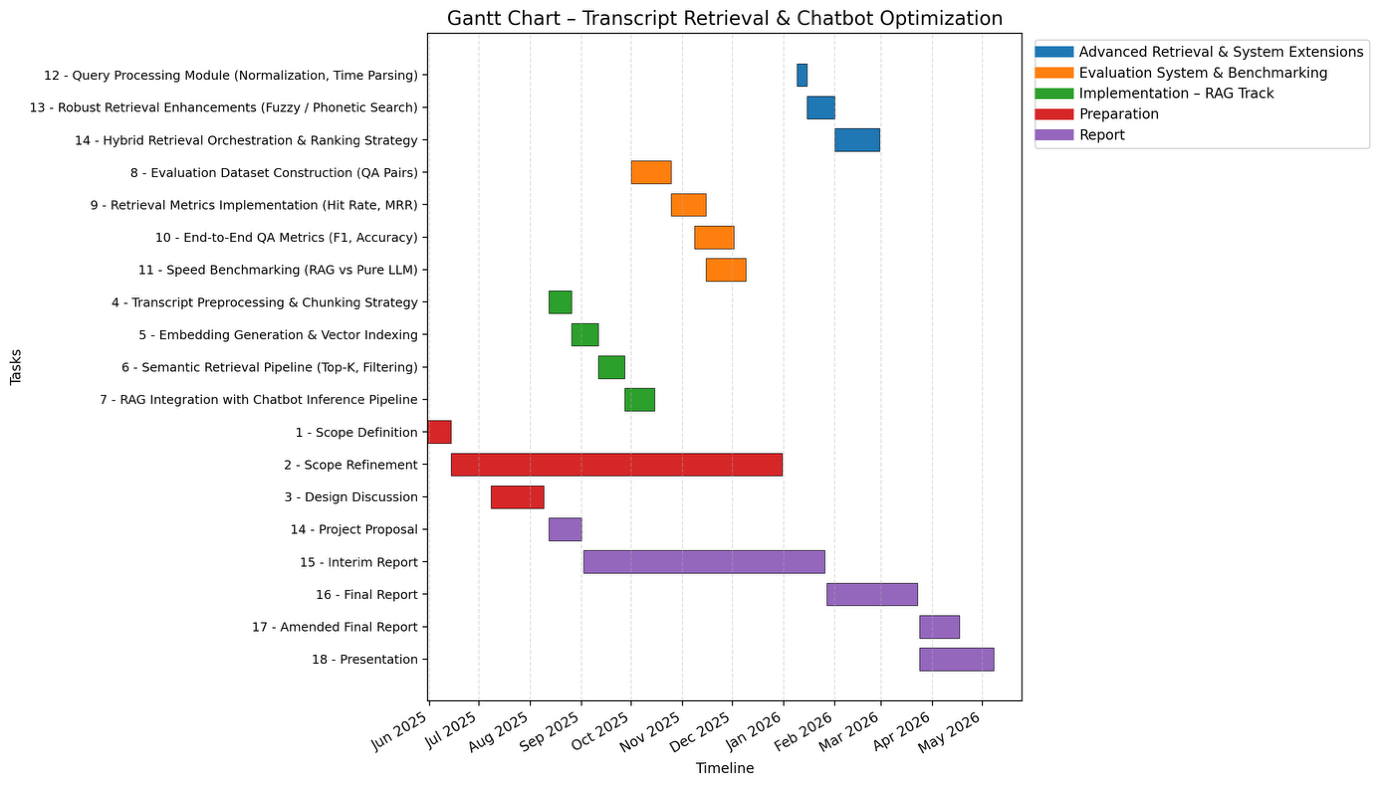
\includegraphics[width=1.0\textwidth]{figures/gantt_chart_representing_the_project_timeline.png}
  \caption{Gantt chart representing the project timeline}
  \label{fig:fig2}
\end{figure}

\begin{table}[H]
  \centering
  \small
  \begin{tabular}{|c|>{\raggedright\arraybackslash}p{0.58\textwidth}|c|c|}
    \hline
    \textbf{Index} & \textbf{Task Name} & \textbf{Start Date} & \textbf{End Date} \\
    \hline
    \multicolumn{4}{|l|}{\textbf{Preparation}} \\
    \hline
    1 & Scope Definition & 31 May 2025 & 14 Jun 2025 \\
    2 & Scope Refinement & 14 Jun 2025 & 31 Dec 2025 \\
    3 & Design Discussion & 8 Jul 2025 & 9 Aug 2025 \\
    \hline
    \multicolumn{4}{|l|}{\textbf{Implementation -- RAG Track}} \\
    \hline
    4 & Transcript Preprocessing \& Chunking Strategy & 12 Aug 2025 & 26 Aug 2025 \\
    5 & Embedding Generation \& Vector Indexing & 26 Aug 2025 & 11 Sept 2025 \\
    6 & Semantic Retrieval Pipeline (Top-K, Filtering) & 11 Sept 2025 & 27 Sept 2025 \\
    7 & RAG Integration with Chatbot Inference Pipeline & 27 Sept 2025 & 15 Oct 2025 \\
    \hline
    \multicolumn{4}{|l|}{\textbf{Evaluation System \& Benchmarking}} \\
    \hline
    8 & Evaluation Dataset Construction (QA Pairs) & 1 Oct 2025 & 25 Oct 2025 \\
    9 & Retrieval Metrics Implementation (Hit Rate, MRR) & 25 Oct 2025 & 15 Nov 2025 \\
    10 & End-to-End QA Metrics (F1, Accuracy) & 8 Nov 2025 & 2 Dec 2025 \\
    11 & Speed Benchmarking (RAG vs Pure LLM) & 15 Nov 2025 & 9 Dec 2025 \\
    \hline
    \multicolumn{4}{|l|}{\textbf{Advanced Retrieval \& System Extensions}} \\
    \hline
    12 & Query Processing Module (Normalization, Time Parsing) & 9 Jan 2026 & 15 Jan 2026 \\
    13 & Robust Retrieval Enhancements (Fuzzy / Phonetic Search) & 15 Jan 2026 & 1 Feb 2026 \\
    14 & Hybrid Retrieval Orchestration \& Ranking Strategy & 1 Feb 2026 & 28 Feb 2026 \\
    \hline
    \multicolumn{4}{|l|}{\textbf{Report}} \\
    \hline
    14 & Project Proposal & 12 Aug 2025 & 1 Sept 2025 \\
    15 & Interim Report & 2 Sept 2025 & 26 Jan 2026 \\
    16 & Final Report & 27 Jan 2026 & 23 Mar 2026 \\
    17 & Amended Final Report & 24 Mar 2026 & 17 Apr 2026 \\
    18 & Presentation & 24 Mar 2026 & 8 May 2026 \\
    \hline
  \end{tabular}
  \caption{Detailed project schedule}
  \label{tab:project-schedule}
\end{table}
